\chapter{Relações (3º Bimestre)}

\section{Variação de grandezas proporcionais}

Una grandeza $A$ is (directly)
proportional to another grandeza $B$ if the value of $A$
can be obtained from the value of $B$ by multiplication by a constant number.
For example, $B$ is a number of boxes and each such box contains $6$
eggs then the total number of eggs is $A = 6 \times B$ so $A$ is proportional
to $B$. If $A$ is actually proportional to $\frac{1}{B}$ we say that $A$ is
inversely proportional to $B$.

\subsection*{Exercício 1}

Indicate whether we have variação de grandezas proporcionais and whether
these are direct or inverse.

\begin{enumerate}
\item The price of tomatoes in a shop is given by the following table:

  \begin{tabular}{c | c}
Tomatoes (kg) & Price (R\$) \\
\hline
0.5 & 2.4 \\
\hline
1 & 4.8 \\
\hline
1.5 & 7.2 \\
\hline
2 & 9.6 \\
\hline
2.5 & 12
\end{tabular}

\item We cut a rope of length $1\text{m}$ into several pieces of equal lengths.
  The following table provides a measure of the length of each piece.

\begin{tabular}{c | c}
number of pieces & length of each piece (\text{cm}) \\
\hline
2 & 50 \\
\hline
3 & 33.33 \\
\hline
4 & 25 \\
\hline
5 & 20 \\
\hline
6 & 16.67 \\
\hline
7 & 14.29 \\
\hline
\end{tabular}

\item The intensity of the current through a $250$ ohm resistor follows
  Ohm's rule. The following table provides the measure of this intensity
  for various voltage values.

\begin{tabular}{c | c}
voltage (V) & current (mA) \\
\hline
4 & 16 \\
\hline
6 & 24 \\
\hline
8 & 32 \\
\hline
10 & 40 \\
\hline
\end{tabular}

\item The pressure of hydrogen gas at fixed temperature follows the
  Boyle-Mariotte law. The following table provides the measure of the pressure
  for various volume of the container.

\begin{tabular}{c | c}
volume (mL) & pressure (kPa) \\
\hline
22 & 106.03 \\
\hline
20.2 & 115.47 \\
\hline
17.4 & 134.06 \\
\hline
14.9 & 156.55 \\
\hline
12.6 & 185.13 \\
\hline
11.1 & 210.14 \\
\hline
\end{tabular}

\item The number of digits to write a natural number in decimal notation.
  The following table provides some examples:

\begin{tabular}{c | c}
natural number & number of digits \\
\hline
5 & 1 \\
\hline
50 & 2 \\
\hline
250 & 3 \\
\hline
500 & 3 \\
\hline
1000 & 4 \\
\hline
5000 & 4 \\
\hline
\end{tabular}

\end{enumerate}

\subsection*{Exercício 2}

The following table provides the pressure of a gas in a fixed volume in function
of the temperature.

\begin{tabular}{c | c}
temperature (°C) & pressure (Pa) \\
\hline
0 & 10000 \\
\hline
25 & 10915 \\
\hline
50 & 11830 \\
\hline
75 & 12746 \\
\hline
100 & 13661 \\
\hline
\end{tabular}

\begin{enumerate}
\item Can the pressure be inversely proportional to the temperature?
\item Is the gas pressure proportional to the temperature in °C?
\item Add a column with the temperature in Kelvin (obtained by adding $273.15$
  to the temperature in °C) and another column with the pressure divided
  by the temperature in Kelvin. What do you notice?
\end{enumerate}

\section{Razão e Porcentagem}

From Wikipedia, a
``Razão é a relação existente entre dois valores de uma mesma grandeza''.
A percentagem é uma medida de razão com base 100 (cem). It is common to
represent a razão as a sector in circular diagram (pie chart). For example
a quarter of a circular diagram represents a razão 1:4 or the percentage
$25\%$.

\subsection*{Exercício 3}

\begin{enumerate}
\item We suppose that unemployment rate in a given country represents one
  twentieth of over 100 millions of people. How many people are unemployed?
  What is the percentage of working people?
\item One month later, the number of unemployed people increases by 5\%.
  How many people are
  now unemployed?
\item The next month, the number of unemployed people
  decreases by 5\%. How many people are unemployed?
\item Assuming that we are still considering 100 millions of people, what
  is the percentage of working people?
\end{enumerate}

\subsection*{Exercício 4}

\begin{enumerate}
\item Complete the rows ``Norte'', ``Nordeste'', ``Sudeste'', ``Sul'', ``Centro-Oeste'' in the following  table from the IBGE. Do the same for the total row
``Brasil''.
\item Determine the percentage of ``Norte'', ``Nordeste'', ``Sudeste'', ``Sul'', ``Centro-Oeste'' with respect to the total population of the Brasil and
  represent this information in a pie chart.
\item We choose one Brasilian citizen randomly. What is the probability that
  he or she comes from Sudeste or Sud?
\end{enumerate}

População recenseada e estimada, segundo as Grandes Regiões e as
Unidades da Federação - 2007
\begin{tabular}{c | c}
Grandes Regiões e Unidades da Federação &
População recenseada e estimada \\
\hline
Brasil
& \\
\hline
Norte &
\\
\hline
Rondônia &
1 453 756 \\
\hline
Acre &
655 385 \\
\hline
Amazonas &
3 221 939 \\
\hline
Roraima &
395 725 \\
\hline
Pará &
7 065 573 \\
\hline
Amapá &
587 311 \\
\hline
Tocantins &
1 243 627 \\
\hline
Nordeste &
\\
\hline
Maranhão & 6 118 995 \\
\hline
Piauí & 3 032 421 \\
\hline
Ceará & 8 185 286 \\
\hline
Rio Grande do Norte & 3 013 740 \\
\hline
Paraíba & 3 641 395 \\
\hline
Pernambuco & 8 485 386 \\
\hline
Alagoas & 3 037 103 \\
\hline
Sergipe & 1 939 426 \\
\hline
Bahia & 14 080 654 \\
\hline
Sudeste &
\\
\hline
Minas Gerais & 19 273 506 \\
\hline
Espírito Santo & 3 351 669 \\
\hline
Rio de Janeiro & 15 420 375 \\
\hline
São Paulo & 39 827 570 \\
\hline
Sul &
\\
\hline
Paraná & 10 284 503 \\
\hline
Santa Catarina & 5 866 252 \\
\hline
Rio Grande do Sul & 10 582 840 \\
\hline
Centro-Oeste &
\\
\hline
Mato Grosso do Sul & 2 265 274 \\
\hline
Mato Grosso & 2 854 642 \\
\hline
Goiás & 5 647 035 \\
\hline
Distrito Federal & 2 455 903 \\
\hline
\end{tabular}

\section{Razões constantes na Geometria: π}

\subsection*{Exercício 5}

Draw circles of diameter $2$, $2.5$, $3$, $3.5$, $4$ centimeters and use a
string and a rule to measure the circumference of these circles (rounded to the
millimeter). Use your calculator to determine the ratio of the circumference
and the radius (rounded to the hundredth)
and organize the result in the following table:

\begin{center}
\begin{tabular}{| c | c  | c | c | c | c |}
\hline
Diameter (cm) & $2$ & $2.5$ & $3$ & $3.5$ & $4$ \\
\hline
Circumference (cm) &  &  &  &  & \\
\hline
$\frac{\text{Circumference}}{\text{Radius}}$ &  &  &  &  &  \\
\hline
\end{tabular}
\end{center}

What can you say about the values of
$\frac{\text{Circumference}}{\text{Diameter}}$? Determine the mean of these
values.

\subsection*{Definition}

The previous exercise suggests that the circumference of a circle is
proportional to its radius. We define
%%
$$
\pi = \frac{\text{Circumference}}{\text{Diameter}}
$$
%%
with $\pi \approx 3.14$. In particular the circumference of a circle of
radius $R$ is
%%
$$l = 2 \times \pi \times R$$
%%
and more generally the length of the perimetor of a sector of $\theta$° of
such a circle is
%%
$$l_\theta = \frac{\theta°}{360°} \times 2 \times \pi \times R$$

\subsection*{Exercício 6}

Calcule una aproximación de

\begin{enumerate}
\item La longitud del círculo central de un terreno de fútbal (radio: $9.15$m).
\item La longitud del arco corespondiente a un radio de $R=2$m y ángulo
$\alpha=35$°.
\end{enumerate}

\subsection*{Exercício 7}

We consider a Cartesian coordinate system and a number $R > 0$.

\begin{enumerate}

\item The Javascript function {\tt Math.random()} returns a
  pseudo-random number $f$ such that $0 \leq f < 1$. For simplicity's sake, we
  assume that $f$ might as well take the value $1$. What is the closed
  interval $I$
  covered by the possible values of $2 \times R \times \left(f - 0.5\right)$?

\item Let $x, y$ be random numbers in $I$. What is the area $A$ covered by
  the possible points $(x,y)$? Express $A$ in function of $R$.

\item The Javascript function {\tt Math.hypot(x, y)} returns the distance
  from the origin $(0,0)$ to the point of coordinates $(x, y)$.
  What is the area $B$ covered by the possible points $(x,y)$ such that
  {\tt Math.hypot(x, y) < R}?

\item Express in function of $A$ and $B$ the probability $p$ that a random
  point $(x,y)$ in $A$ belongs to $B$.

\item The following Javascript program count the number {\tt NInside} of
  points inside $B$ among
  {\tt NAttempts = 100000} random points inside $A$.
  How does the ratio {\tt NInside / NAttempts} relate to the probability $p$?

\begin{lstlisting}
  var R = 10, NAttempts = 100000, NInside = 0;
  function randomCoord() { return (Math.random() - .5) * 2 * R; }
  for (var i = 0; i < NAttempts; i++) {
    if (Math.hypot(randomCoord(), randomCoord()) < R) NInside++;
  }
  4 * NInside / NAttempts;
\end{lstlisting}

\item Try to execute it in your favorite browser so that you obtain the
  value {\tt 4 * NInside / NAttempts}. What do you notice?

\item Propose an expression of $B$ in function of $R$ and $\pi$.

\end{enumerate}

\section{Solução dos exercícios}

\subsection*{Exercício 1}

\begin{enumerate}
\item The price of the tomatoes in $R\$$
  is directly proportional to the kilos bought (by a factor $4.8$).

\item The length of each piece is given by $100\text{cm}$ divided by the number
  of pieces, so it is inversely proportional to the number
  of pieces.

\item The current in mA is directly proportional to the voltage
  (by a factor $4$)
\item The pressure seems inversely proportional to the volume.
  The factor is approximately 2332.6.

  \begin{tabular}{c | c | c}
volume (mL) & pressure (kPa) & $\text{volume} \times \text{pressure}$ \\
\hline
22 & 106.03 & 2332.66 \\
\hline
20.2 & 115.47 & 2332.494 \\
\hline
17.4 & 134.06 & 2332.644 \\
\hline
14.9 & 156.55 & 2332.595 \\
\hline
12.6 & 185.13 & 2332.638 \\
\hline
11.1 & 210.14 & 2332.554 \\
\hline
\end{tabular}

\item This is not inversely proportional: the number of digits increases
  when the natural number becomes larger (and both values are positive).
  This is not directly proportional
  either: when we multiply $5$ by a factor $1000$, the number of digits is
  only multiplied by $4$.

\end{enumerate}

\subsection*{Exercício 2}

\begin{enumerate}
\item No: in the table we see that the pressure increases when the temperature
  increases.
\item No: when we multiply a temperature of $25$°C by 2, 3, or 4 the
  pressure is not multiplied by the same factor.
\item We obtain the following table, suggesting that the
  pressure in Pascal is proportional to the temperature in Kelvin
  (by a factor 36.61).

\begin{tabular}{c | c | c | c}
  temperature (°C) & temperature (K) & pressure (Pa) &
  pressure (Pa) divided by temperature (K)
  \\
\hline
0 & 273.15 & 10000 & 36.6099 \\
\hline
25 & 298.15 & 10915 & 36.6091 \\
\hline
50 & 323.15 & 11830 & 36.6084 \\
\hline
75 & 348.15 & 12746 & 36.6107 \\
\hline
100 & 373.15 & 13661 & 36.6099 \\
\hline
\end{tabular}

\end{enumerate}

\subsection*{Exercício 3}

\begin{enumerate}
\item
  $100 / 20 = 5$ millions of people are unemployed.
  The percentage of working people is $100-5=95\%$.
\item
  $5 + \frac{5}{100} \times 5 = 5.25$ millions of people are now unemployed.
\item
  $5.25 - \frac{5}{100} \times 5.25 = 4.9875$ millions of people are now
  unemployed.
\item There are $100 - 4.9875 = 95.0125\%$ working people.
\end{enumerate}

\subsection*{Exercício 4}

\begin{enumerate}
\item \begin{tabular}{c | c | c}
Grandes Regiões e Unidades da Federação &
População recenseada e estimada &
Porcentagem \\
\hline
Brasil
& 183 987 291
& 100\% \\
\hline
Norte &
14 623 316 &
7.95\% \\
\hline
Nordeste &
51 534 406 &
28\% \\
\hline
Sudeste &
77 873 120 &
42.33\% \\
\hline
Sul &
26 733 595 &
14.53\% \\
\hline
Centro-Oeste &
13 222 854 &
7.19\% \\
\hline
\end{tabular}

\item
  \begin{center}
    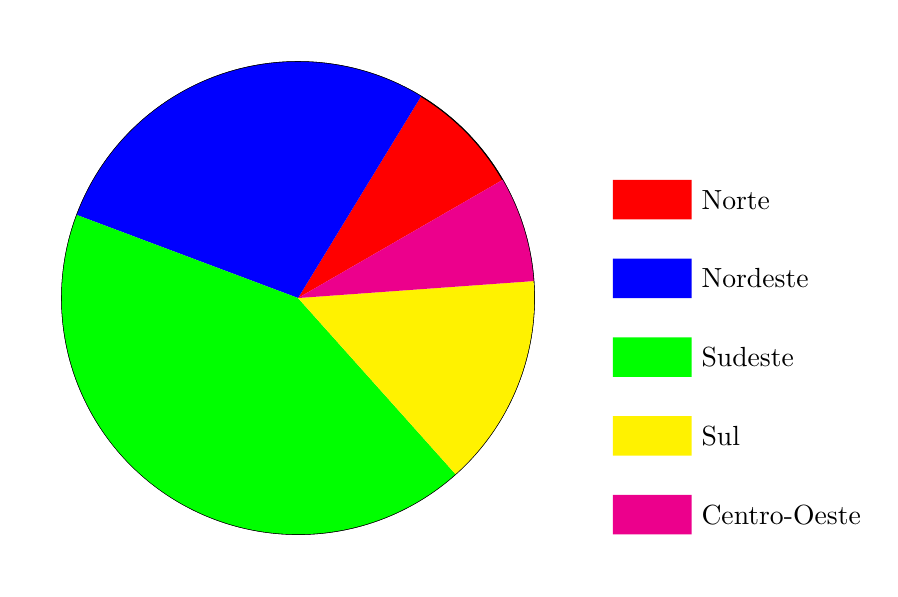
\begin{tikzpicture}
      \begin{scope}[shift={(4,1)}]
        \path[fill=red] (0,0) -- (1,0) -- (1,.25)node[right]{Norte} -- (1,.5) -- (0,.5) -- cycle;
      \end{scope}
      \begin{scope}[shift={(4,0)}]
        \path[fill=blue] (0,0) -- (1,0) -- (1,.25)node[right]{Nordeste} -- (1,.5) -- (0,.5) -- cycle;
      \end{scope}
      \begin{scope}[shift={(4,-1)}]
        \path[fill=green] (0,0) -- (1,0) -- (1,.25)node[right]{Sudeste} -- (1,.5) -- (0,.5) -- cycle;
      \end{scope}
      \begin{scope}[shift={(4,-2)}]
        \path[fill=yellow] (0,0) -- (1,0) -- (1,.25)node[right]{Sul} -- (1,.5) -- (0,.5) -- cycle;
      \end{scope}
      \begin{scope}[shift={(4,-3)}]
        \path[fill=magenta] (0,0) -- (1,0) -- (1,.25)node[right]{Centro-Oeste} -- (1,.5) -- (0,.5) -- cycle;
      \end{scope}

      \draw (0,0) circle(3)[color=black];
      \begin{scope}[rotate={30}]
      \begin{scope}[rotate={0}]
        \path[fill=red] (0,0) -- (3,0) arc(0:28.62:3);
      \end{scope}
      \draw (0,0) circle(3)[color=black];
      \begin{scope}[rotate={28.62}]
        \path[fill=blue] (0,0) -- (3,0) arc(0:100.8:3);
      \end{scope}
      \begin{scope}[rotate={129.42}]
        \path[fill=green] (0,0) -- (3,0) arc(0:152.388:3);
      \end{scope}
      \begin{scope}[rotate={281.808}]
        \path[fill=yellow] (0,0) -- (3,0) arc(0:52.308:3);
      \end{scope}
      \begin{scope}[rotate={334.116}]
        \path[fill=magenta] (0,0) -- (3,0) arc(0:25.884:3);
      \end{scope}
      \end{scope}
   \end{tikzpicture}
  \end{center}
\item
  Sudeste and Sud represents
  $\frac{26733595+77873120}{183987291} = \frac{34868905}{61329097}
  \approx 56\%$ of the population so there is more than one chance over two.
\end{enumerate}

\subsection*{Exercício 5}

\begin{center}
\begin{tabular}{| c | c  | c | c | c | c |}
\hline
Diameter (cm) & $2$ & $2.5$ & $3$ & $3.5$ & $4$ \\
\hline
Circumference (cm) & $6.3$ & $7.9$ & $9.4$ & $11$ & $12.6$ \\
\hline
$\frac{\text{Circumference}}{\text{Radius}}$ & $3.15$ & $3.16$ & $3.13$ &
$3.14$ & $3.15$ \\
\hline
\end{tabular}
\end{center}

We notice that $\frac{\text{Circumference}}{\text{Radius}}$ is almost constant
with a mean of $\frac{3.15+3.16+3.13+3.14+3.15}{5} = 3.146$.


\subsection{Exercício 6}

\begin{enumerate}
\item $2 \times \pi \times 9.15 \approx 57.5$m.
\item $2 \times \pi \times 2 \times \frac{35}{360} \approx 1.22$m.
\end{enumerate}

\subsection*{Exercício 7}

\begin{enumerate}

\item We have $0 \leq f \leq 1$ so $-0.5 \leq f - 0.5 \leq 0.5$,
  $-R \leq 2 \times R \times \left(f - 0.5 \right) \leq R$. So
  $I = {[-R, R]}$

\item $A$ is a square of side $2R$ centered at the origin.
  We have $A = {2R} \times {2R} = 4R^2$.

\item $B$ is the circle of radius $R$ and center the origin.

\item $\frac{B}{A}$

\item {\tt NInside/NAttempts} should approximate the probability $p$.

\item {\tt 4 * NInside / NAttempts} is very close to $\pi$.

\item This suggests that the area of the circle is
  $B = \frac{A \times \pi}{4} = \pi R^2$.

\end{enumerate}
